\documentclass[a4paper,11pt]{article}
\usepackage{amsmath,amsthm,amsfonts,amssymb,amscd,amstext,vmargin,graphics,graphicx,tabularx,multicol} 
\usepackage[francais]{babel}
\usepackage[utf8]{inputenc}  
\usepackage[T1]{fontenc} 
\usepackage{pstricks-add,tikz,tkz-tab,variations}
\usepackage[autolanguage,np]{numprint} 

\setmarginsrb{1.5cm}{0.5cm}{1cm}{0.5cm}{0cm}{0cm}{0cm}{0cm} %Gauche, haut, droite, haut
\newcounter{numexo}
\newcommand{\exo}[1]{\stepcounter{numexo}\noindent{\bf Exercice~\thenumexo} : \marginpar{\hfill /#1}}
\reversemarginpar


\newcounter{enumtabi}
\newcounter{enumtaba}
\newcommand{\q}{\stepcounter{enumtabi} \theenumtabi.  }
\newcommand{\qa}{\stepcounter{enumtaba} (\alph{enumtaba}) }
\newcommand{\initq}{\setcounter{enumtabi}{0}}
\newcommand{\initqa}{\setcounter{enumtaba}{0}}

\newcommand{\be}{\begin{enumerate}}
\newcommand{\ee}{\end{enumerate}}
\newcommand{\bi}{\begin{itemize}}
\newcommand{\ei}{\end{itemize}}
\newcommand{\bp}{\begin{pspicture*}}
\newcommand{\ep}{\end{pspicture*}}
\newcommand{\bt}{\begin{tabular}}
\newcommand{\et}{\end{tabular}}
\renewcommand{\tabularxcolumn}[1]{>{\centering}m{#1}} %(colonne m{} centrée, au lieu de p par défault) 
\newcommand{\tnl}{\tabularnewline}

\newcommand{\bmul}[1]{\begin{multicols}{#1}}
\newcommand{\emul}{\end{multicols}}

\newcommand{\trait}{\noindent \rule{\linewidth}{0.2mm}}
\newcommand{\hs}[1]{\hspace{#1}}
\newcommand{\vs}[1]{\vspace{#1}}

\newcommand{\N}{\mathbb{N}}
\newcommand{\Z}{\mathbb{Z}}
\newcommand{\R}{\mathbb{R}}
\newcommand{\C}{\mathbb{C}}
\newcommand{\Dcal}{\mathcal{D}}
\newcommand{\Ccal}{\mathcal{C}}
\newcommand{\mc}{\mathcal}

\newcommand{\vect}[1]{\overrightarrow{#1}}
\newcommand{\ds}{\displaystyle}
\newcommand{\eq}{\quad \Leftrightarrow \quad}
\newcommand{\vecti}{\vec{\imath}}
\newcommand{\vectj}{\vec{\jmath}}
\newcommand{\Oij}{(O;\vec{\imath}, \vec{\jmath})}
\newcommand{\OIJ}{(O;I,J)}


\newcommand{\reponse}[1][1]{%
\multido{}{#1}{\makebox[\linewidth]{\rule[0pt]{0pt}{20pt}\dotfill}
}}

\newcommand{\titre}[5] 
% #1: titre #2: haut gauche #3: bas gauche #4: haut droite #5: bas droite
{
\noindent #2 \hfill #4 \\
#3 \hfill #5

\vspace{-1.6cm}

\begin{center}\rule{6cm}{0.5mm}\end{center}
\vspace{0.2cm}
\begin{center}{\large{\textbf{#1}}}\end{center}
\begin{center}\rule{6cm}{0.5mm}\end{center}
}



\begin{document}
\pagestyle{empty}
\titre{Interrogation sur les statistiques}{Nom :}{Prénom :}{Classe}{Date}

\begin{flushleft}
\begin{tabular}{|m{9.5cm}|m{1.25cm}|m{1.25cm}|m{1.25cm}|m{1.25cm}|m{1.25cm}|}
\hline 
\textbf{Compétences} & \begin{center}
\textbf{N.E.}
\end{center} & \begin{center}
\textbf{M.I.}
\end{center} & \begin{center}
\textbf{M.F.}
\end{center}  & \begin{center}
\textbf{M.S.}
\end{center} & \begin{center}
\textbf{T.B.M.}
\end{center} \\ 
\hline 
Je dois savoir  lire et interpréter des données sous forme de données brutes, de tableau, de diagramme (diagramme en bâtons, diagramme circulaire, histogramme) &  &  & & &\\
\hline 
Je dois savoir calculer des effectifs, des fréquences (liste, tableau, graphique, tableur) &  &  & & &\\
\hline
Je dois savoir calculer une moyenne pondérée &  &  & & &\\
\hline
\end{tabular} 
\end{flushleft}

\textit{N.E = Non évalué ; M.I. = Maîtrise insuffisante ; M.F. = Maîtrise fragile ; M.S. = Maîtrise satisfaisante ; T.B.M. = Très bonne maîtrise}\\

\exo{8}

L'histogramme ci-dessous donne la répartition des élèves d'un collège en fonction du temps qu'il mettent à venir au collège.

\begin{center}
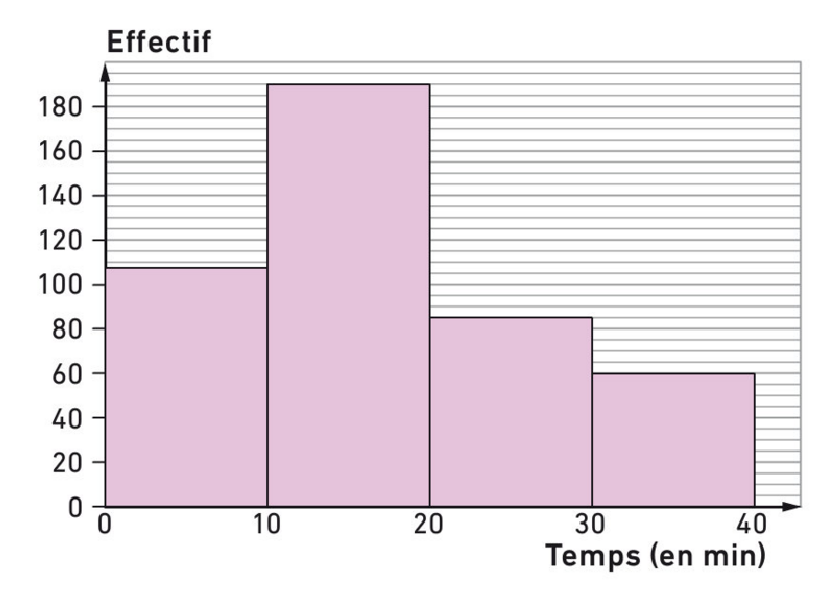
\includegraphics[scale=0.9]{interro2.eps} 
\end{center}

Voici un tableau qui représente la situation :\\

\renewcommand{\arraystretch}{2}

\begin{tabular}{|c|c|c|c|c|}
\hline 
Temps (en min) & \hspace*{0.3cm} [0;10[ \hspace*{0.3cm}& \hspace*{0.3cm} [10;20[ \hspace*{0.3cm} & \hspace*{0.3cm} [20;30[ \hspace*{0.3cm} & \hspace*{0.3cm} [30;40[ \hspace*{0.3cm} \\ 
\hline 
Effectifs & 107  &  &  &   \\ 
\hline 
Effectifs cumulés croissants &  &  &  &   \\ 
\hline 
Fréquences (en pourcentage) &  &  &  &  \\ 
\hline 
\end{tabular} 

\vspace*{0.4cm}


\q Quelles sont les valeurs extrêmes de la série statistique ?\\


\q Compléter la ligne des effectifs et des effectifs cumulés du tableau ci-dessus. (sans justification)\\



\q Combien d'élèves mettent plus de 30 min \textit{(30 min inclus)}, pour venir au collège ? \\


\q Compléter la ligne des fréquences en pourcentage. (sans justification)\\


\q Quelle est la fréquence en pourcentage du nombre d'élèves qui mettent au plus 20 min \textit{(20 min exclu)}, pour venir au collège ? Justifier votre réponse par un calcul. \\


\q Quelle est la fréquence en pourcentage du nombre d'élèves qui mettent au moins 10 min \textit{(10 min inclus)}, pour venir au collège ? Justifier votre réponse par un calcul. \\

\q En combien de temps en moyenne, un élève met-il pour venir au collège ? \\

\noindent  \reponse[33]\\ 



\newpage


\exo{2}

En réalité, le débit d'écoulement d'un même sablier n'est pas constant.\\
Dans une usine où on fabrique des sabliers, on prend un sablier au hasard et on teste plusieurs fois le temps d'écoulement de ce sablier.\\

Voici les différents temps récapitulés dans le tableau suivant :\\

   \includegraphics[scale=1]{sablier.eps} \\
   
 
 Un sablier est mis en vente s'il vérifie les trois conditions ci-dessous, sinon il est éliminé :\\
 
\noindent • La différence entre le temps maximum et le temps minimum est inférieure à 20 s.\\
• 50 \% des temps sont inférieurs à 2 min 30 s.\\
• La moyenne des temps est comprise entre 2 min 28 s et 2 min 32 s.\\

Le sablier testé sera-t-il éliminé ?\\

\noindent  \reponse[20]\\ 
\end{document}
